% Extracted from linearApproximation.tex, problem #7
\begin{problem}
The graph of a function $f$ is given below.
    % \begin{image}
    %  \includegraphics{figure3.png}
    %\end{image}
    	  \begin{center}
		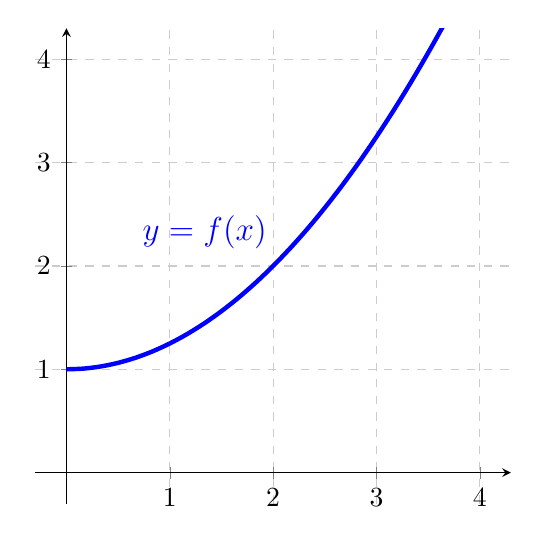
\begin{tikzpicture}
			\begin{axis}[
				xmin=-0.3, xmax=4.3, ymin=-0.3,ymax=4.3,    
				axis lines =middle, 
				every axis y label/.style={at=(current axis.above origin),anchor=south},
				every axis x label/.style={at=(current axis.right of origin),anchor=west},
				xtick={0,...,4}, ytick={0,...,4},
				grid=major, width=3in, height = 3in,
				grid style={dashed, gray!40}
				]
				\addplot[color=blue, ultra thick, smooth, domain=0:4]{(1/4)*x^2+1} node[pos=0.4, color=blue, above left]{\large{$y=f(x)$}};				

			\end{axis}
		\end{tikzpicture}
	\end{center}
%part a
\begin{enumerate}
\item Given that $f'(2)=1$, find the linear approximation $L$ to the function $f$ at $a=2$.
	\WkstHop[2]

\begin{freeResponse}
$L(x)=f(2)+f'(2)(x-2)=2+(x-2)=x$
\end{freeResponse}

%part b
\item Sketch the graph of $L$ in the figure above.
\begin{freeResponse}
    \begin{image}
      \includegraphics[scale = .7]{figure4.png}
    \end{image}
\end{freeResponse}

%part c
\item Use the linear approximation $L$ to estimate the value of $f(3)$.  Is this an underestimate or overestimate?  \textbf{EXPLAIN}.
	\WkstHop[2]
\begin{freeResponse}
$f(3)\approx L(3)=3$.  It is an underestimate because $f$ is concave up on the interval $(2, 3)$.
\end{freeResponse}

%part d
\item When $x$ changes from $a=2$ to $a+\Delta x=3$, the change in the {\bf function} $y=f(x)$, $\Delta y$, is given by $\Delta y=f(a+ \Delta x)-f(a)$.  Draw and label $\Delta y$ and $\Delta x$ in the figure above.


\begin{freeResponse}
   \begin{image}
      \includegraphics[scale = .6]{figure5.png}
    \end{image}
\end{freeResponse}

%part e
\item When $x$ changes from $a=2$ to $a+ \Delta x=3$, the change in the {\bf linear approximaton}, $dy$, is given by $dy=L(a+\Delta x)-L(a)=f'(a)\Delta x$.  Draw and label $L(x)$, $dx$ and $dy$ (differential) in the figure above.
%   \begin{image}
%      \includegraphics[scale = .7]{figure6.png}
%    \end{image}

\begin{freeResponse}
   \begin{image}
      \includegraphics[scale = .7]{figure7.png}
    \end{image}
\end{freeResponse}

\end{enumerate}
\end{problem}
